%
\section{Moving converter to OPA}

Make degrader of CH2 , 24mm thick) and move the converter to OPA .
\begin{itemize}
\item
  Generate 10M events
\item 
  The simulated range of cos(theta) is [0,0.45] - dataset family rpc07b0
\end{itemize}

\begin{figure}[H]
  \begin{tikzpicture}
    \node[anchor=south west,inner sep=0] at (0,0.) {
      % \node[shift={(0 cm,0.cm)},inner sep=0,rotate={90}] at (0,0) {}
      \makebox[\textwidth][c] {
        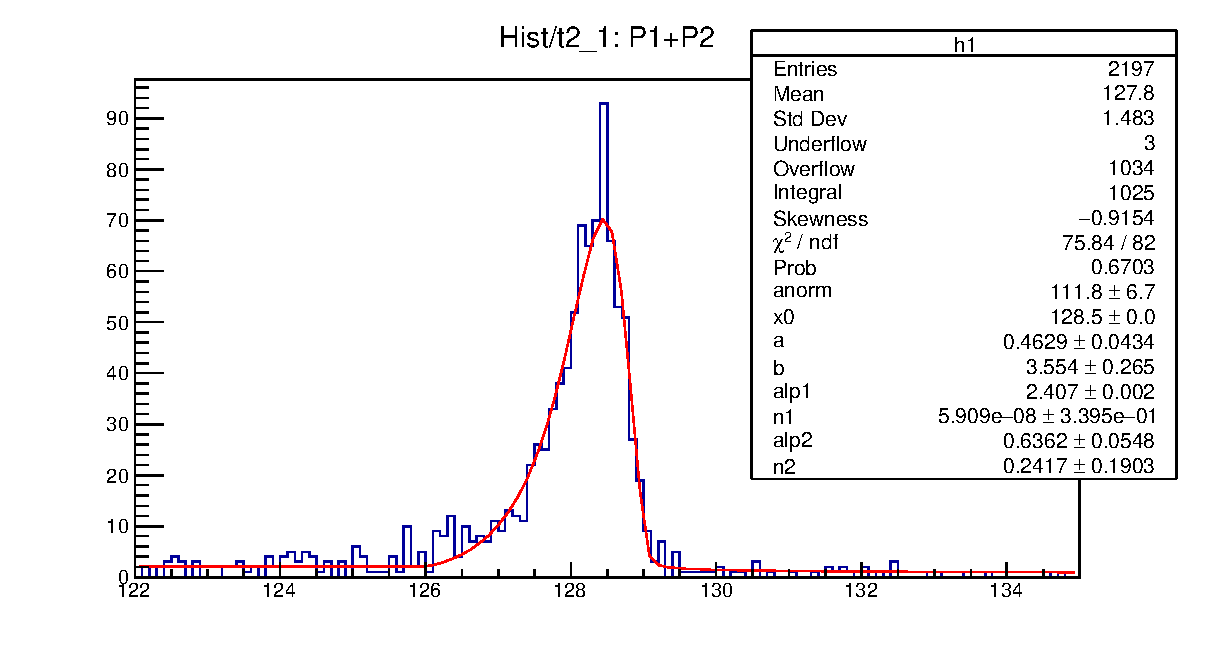
\includegraphics[width=0.95\textwidth]{pdf/pipenu_rpc07b0s51r0100_drpc_ana_t2_1_smom_1_fit}
      }
    };
    % \node [text width=8cm, scale=1.0] at (14.5,0.5) {$\mu_B$, expected background mean};
    % \node [text width=8cm, scale=1.0, rotate={90}] at (1.5,7.5) { $S_{D}$, ``discovery'' signal strength  };
  \end{tikzpicture}
  \caption{
    \label{figure:t2_1_smom_0}
    Sum of the two reconstructed track momenta and its fi.t 2cm wide converter in OPA
  }
  \label{figure:event_display}
\end{figure}


%%% Local Variables:
%%% mode: latex
%%% TeX-master: t
%%% End:
